\documentclass{beamer}

\usepackage{ctex}
\usepackage{graphicx}
\usepackage{animate}

\usetheme{Pittsburgh}

\graphicspath{{pictures/}}

% \usecolortheme{dove} % 

% 最传统 warsaw Pittsburgh Singapore Malmoe Boadilla


\title[Latex使用模板]{打算构建一个Latex使用模板}
\subtitle[课程]{职业生涯的一小课程}
\author[Dong Yu]{{\small 学生 董昱 \\ 导师 闫慧敏 副研究员}}
\date[\today]{\today}
\institute[中科院地理所]{中国科学地理科学与资源研究所\par 中国科学院大学}
% \titlegraphic{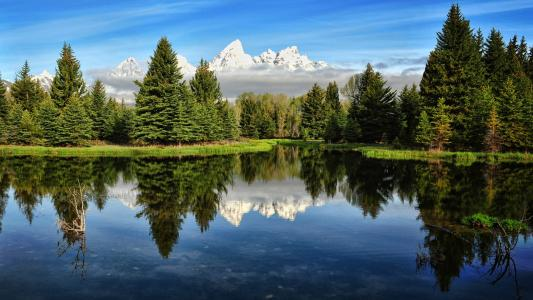
\includegraphics[width=0.17\textwidth]{image.jpg}}

\begin{document}
	
	% 标题页帧
	\frame{\titlepage}

	\begin{frame}[label = outline]
		\frametitle{汇报内容}
		% \tableofcontents[part=1,pausesections]
		\tableofcontents
	\end{frame}

	\section{基本用法}

	% 普通帧
	\begin{frame}[c] % c表示对齐方式
		\frametitle{讲述你的故事}
		\framesubtitle{也许会用到这个副标题}
		The is the content
		
		\hyperlink{outline}{\beamergotobutton{超链接}}
	\end{frame}

	\section{gif动画}
	
	\subsection{带控制按钮}
	
	\begin{frame}[c] % c表示对齐方式
		\frametitle{动画}

		\animategraphics[autoplay,loop,controls,width=.7\textwidth,height=.7\textheight]{1}{test}{0}{2}  

	\end{frame}

	\subsection{不带控制按钮}

	\begin{frame}[c]
		\frametitle{动画}

		\animategraphics[autoplay,loop,width=.7\textwidth,height=.7\textheight]{5}{test}{0}{2}

	\end{frame}

	\subsection{基本slide控制}

	\begin{frame}{动画效果展示}  
		\onslide<1>{只有第一部}  
		
		\onslide<2->{第二部之后}  
		
		\onslide<1,3>{第1,3两步}  
		
		\textbf<3>{只在第三步加粗} 
	\end{frame}  

	\begin{frame}{动画显示}  
	\begin{itemize}  
		\item<1->显示列表一  
		
		\item<2->显示列表二  
		
		\item<3->显示列表三  
		
	\end{itemize}  
	\end{frame}  

	\begin{frame}  
		\begin{itemize}[<+->]  
			\item 开始显示  
			\item 其次显示  
			其次显示  
			
			其次显示  
			其次显示  其次显示  
			\item 最后显示  
		\end{itemize}  
	\end{frame}  

	\begin{frame}{动画显示}  
		\begin{itemize}  
			\item<+-| structure@+>显示列表一  
			
			\item<2-| alert@+>显示列表二  
			
			\item<3->显示列表三  
			
		\end{itemize}  
	\end{frame}

	\section{其他功能}
	
	\begin{frame}
		\begin{columns}
			\column{.5\textwidth}
			First column text and/or code
			\column{.5\textwidth}
			Second column text and/or code
		\end{columns}
	\end{frame}

\end{document}